\definecolor{royalblue}{RGB}{65,105,225}
\definecolor{firebrick}{RGB}{178,34,34}
\definecolor{darkgreen}{RGB}{0,100,0}
\begin{figure}[t]
\centering
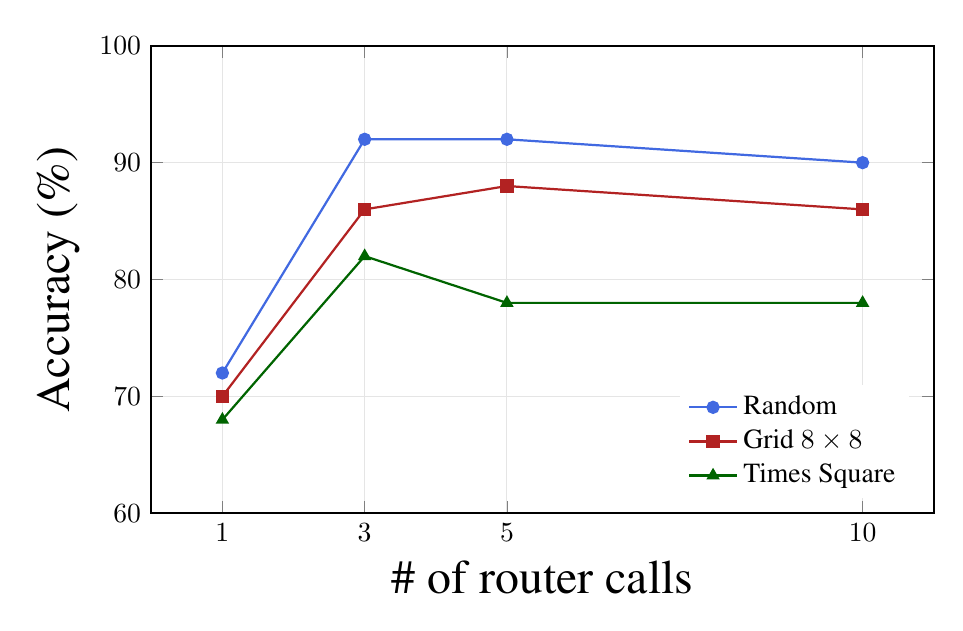
\begin{tikzpicture}[font=\fontfamily{ptm}\selectfont]
\begin{axis}[
    width=0.95\columnwidth, height=0.62\columnwidth,
    xlabel={\# of router calls}, ylabel={Accuracy (\%)},
    label style={font=\LARGE\fontfamily{ptm}\selectfont},
    tick label style={font=\fontfamily{ptm}\selectfont},
    legend style={draw=none, font=\fontfamily{ptm}\selectfont},
    xtick={1,3,5,10},
    xmin=0, xmax=11, ymin=60, ymax=100,
    legend pos=south east, legend cell align={left},
    grid=both, grid style={gray!20}, thick, mark size=2pt,
]
\addplot[royalblue, mark=*] coordinates {(1,72.0) (3,92.0) (5,92.0) (10,90.0)};
\addlegendentry{Random}
\addplot[firebrick, mark=square*] coordinates {(1,70.0) (3,86.0) (5,88.0) (10,86.0)};
\addlegendentry{Grid $8\times8$}
\addplot[darkgreen, mark=triangle*] coordinates {(1,68.0) (3,82.0) (5,78.0) (10,78.0)};
\addlegendentry{Times Square}
\end{axis}
\end{tikzpicture}
\caption{Router-turn ablation: PER accuracy (\%) on the multi-step reasoning tasks as the router-turn budget varies.}
\label{fig:ablation_router_turns}
\end{figure}
